% ----------------------------------------------------
% Institute of Medical Informatics
% University of Luebeck
%
% Version 0.4
%
% ----------------------------------------------------

\documentclass[
%a4paper,
12pt,
headsepline,
bibliography=totoc,
twoside=semi,
fleqn
]{scrartcl}

\usepackage{pgf}
\usepackage{ucs}
%\usepackage[latin1]{inputenc}
\usepackage[utf8]{inputenc}
%\usepackage[pdftex]{graphicx}
%\usepackage{color}
%\usepackage{german}
\usepackage{subfigure}
\usepackage{booktabs}
\usepackage{float}
\usepackage{wrapfig}
\usepackage{amsmath}

\graphicspath{{./images/}}
%% LAYOUT:

\renewcommand{\descfont}{\bfseries}
\renewcommand{\sectfont}{\bfseries}

\addtolength{\topmargin}{-1.5cm}
\addtolength{\textheight}{1.5cm}

\setkomafont{captionlabel}{\bfseries\footnotesize}
\setkomafont{caption}{\footnotesize}
\renewcommand{\headfont}{\bfseries}
\renewcommand{\figurename}{Fig.}
\renewcommand{\tablename}{Table}

\renewcommand*{\titlepagestyle}{empty}

\usepackage[automark]{scrlayer-scrpage}
\pagestyle{scrheadings}
\clearscrheadfoot
\rehead{\headmark} 
\lehead{\pagemark} 
\lohead{\headmark} 
\rohead{\pagemark}

\definecolor{Ocean}{cmyk}{1,0,0.2,0.78}
\definecolor{Grey}{cmyk}{0,0,0,0.6}

\usepackage{natbib}
\bibpunct{[}{]}{;}{a}{}{,}

\begin{document}

%==================================================
% TITLE PAGE
% -------------------------------------------------

\setlength{\headheight}{0pt}

\titlehead{
 \flushleft{
\includegraphics[width=0.7\textwidth]{Logo_Inst_MedInformatik_En_P309}}\\[-3.5ex]
 \centering
}

\subject{
\large{
 \vspace{0ex}
 \textnormal{Seminar}\\[1ex] 
 Medical Image Computing and e-Health\\[1ex]
 \textnormal{WS 2020/2021}\\[8ex]
}}

\title{
 \huge{\textcolor{Ocean}{Automatic Detection and Segmentation of Brain Tumor Using Random Forest Approach}}\\[5ex]
}

\author{
 \large{\textbf{Leonard Brenk}}\\
 \large{Matr.-Nr.: 697947, Computer Science}\\[5ex]
 \large{Supervisor}\\
 \large{Marja Fleitmann}\\[8ex]
}

\date{
 \large{Lübeck, \today}
 \pgfdeclareimage{university-slogan}{./images/Slogan_Uni_Luebeck_CMYK}
 \begin{pgfpicture}{0cm}{4cm}{14cm}{1.0cm}
 \pgfputat{\pgfpoint{10cm}{0cm}}{\pgfbox[left,bottom]{\pgfuseimage{university-slogan}}}
 \color {white}
% \pgfputat{\pgfpoint{12.3cm}{0.4cm}}{\pgfbox[right,center]{ \insertshorttitle}} 
 \end{pgfpicture}
}


%============================CONTENT=========================

\maketitle
\newpage
\setcounter{page}{1}
\setlength{\headheight}{58pt}

%==================================================

\tableofcontents
\newpage

%==================================================
% TEXT
% -------------------------------------------------

\section{Motivation\label{sec:sec1}}
The detection and treatment of tumors is a very complex and challenging task. Finding mutating cells and preventing them from spreading is a complicated task. Usually, tumors occur nested in non-affected tissues, which makes their discovery and treatment heavily challenging. The current state of technology operating in that field has complications filtering the negative cells out and segmenting the pure tumor completely. Due to the variety of anatomical structures and how they can differ from person to person, even for a trained professional, it takes a lot of time to detect and fully segment a tumor in MRI scans. Therefore not only are the needed financial and personal requirements greatly inefficient, but also the outcome might be flawed and incomplete based on the individual know-how of the experts.\\

Seeing that finding the tumor in an early stage has the highest impact and can facilitate and enhance the treatment, the detection is the key to success. The paper written by Zoltán Kapás in 2016 captures an experiment regarding this topic. It carries out a Random Forest(RDF) based Machine Learning(ML) technique using multispectral MRI volumes. Training an algorithm to find and segment tumor cells on MRI scans reliably can, due to its large resources in time and memory, possibly perform on a higher level than multiple experts, as Kapás states. Before analyzing the data, it must undergo several pre-processing steps to be suitable for the application in Binary Decision Trees(BDT). Furthermore, after the employment of RDF, the data is post-processed and then analyzed. In order to illustrate the accuracy of a decision, the authors applied a Dice Score. Thereby RDF can be compared and graded. The ML method used in this paper belongs to the supervised learning techniques, which means that the outcome of data the machine is trained with is already known and can be used to adjust and optimize the parameters.\\

The paper presents initial outcomes and recommendations regarding a complex brain tumor detection and segmentation system and its future implementation in a clinical context.

%--------------------------------------------------

\section{Introduction BDT and RDF\label{sec:sec2}}
In this section, the essential basics regarding BDT and RDF and their implementation are being explained and discussed.

 \subsection{Binary Decision Trees\label{sec:sec2-1}}

 \subsubsection{General\label{sec:sec2-1-1}}
 A BDT is trained and employed in order to make a decision based on an input vector. It consists of multiple levels of two-way decisions until it reaches a leaf node at the end, classifying the vector into a certain class. A BDT can be used to either deploy data into classes or predict values in the future using regression. However, this paper will concentrate on the ability to assign a label to a vector. 

 \begin{figure}[H]
 \centering 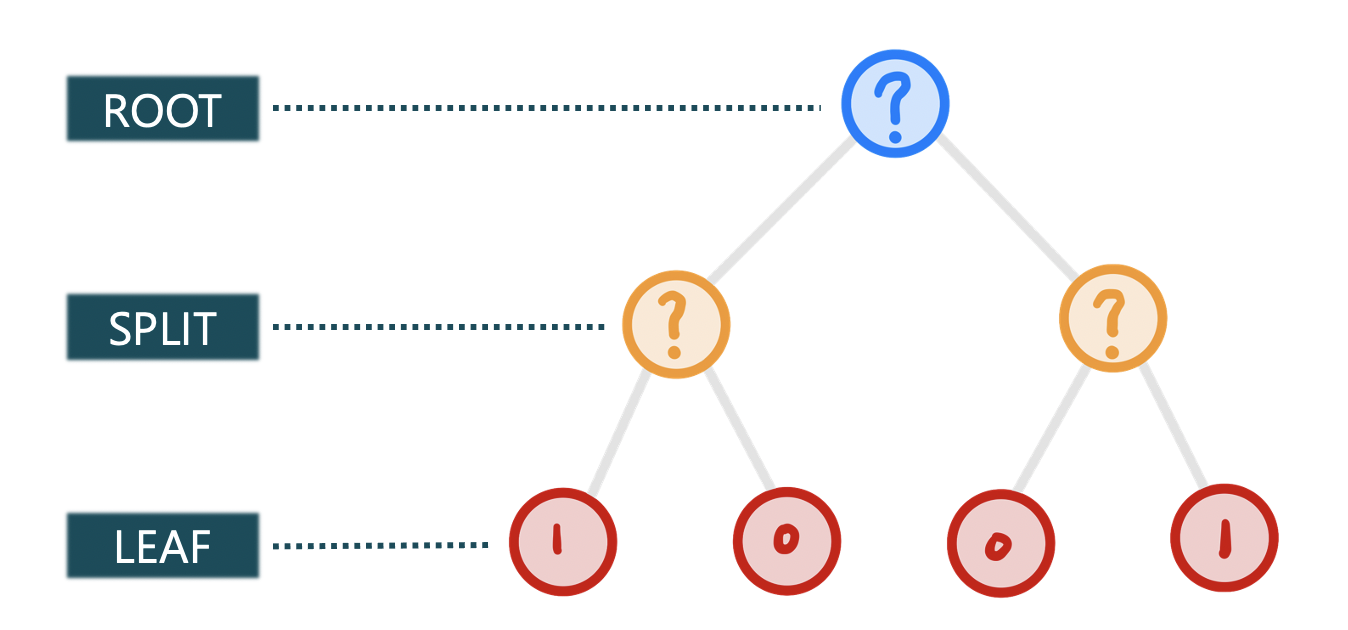
\includegraphics[scale=0.55]{BDT1.png}\label{fig:fig1}
 \caption{The structure of a BDT. Usually there are multiple levels of split nodes.}
 \end{figure}

 The root node is the starting point of a BDT. In order for a BDT to reach a decision, it goes through several inner decision nodes, which divide the data into two subgroups and forwards them to the next node. At each split node, the data is divided again as long as the data subset decisions are distinguishable. If the decisions are unilateral, a leaf node is created. Such leaf nodes are then attributed to a class, also called a label. Thereby an inserted data vector can be classified. 

 \subsubsection{Building a BDT\label{sec:sec2-1-2}}
 A BDT can, amongst other options, be built from a table that contains multiple attributes and a column for the individual decision of that data row. When building a BDT, a cycle is implemented recursively. The data is be divided into two subgroups at a time. Then each subgroup is again divided into two subgroups. In the end, there are as many subgroups as it takes to classify every single data vector correctly. The cycle starts with a given data set. For any first split, an attribute needs to be picked, which the data is split with. Having decided upon that attribute, a threshold is set to decide whether a vector is forwarded to the left or right child node - depending on whether its value is higher or smaller than the threshold. Using the threshold, the complete data set can then be divided into two subgroups. Now each subgroup is considered individually, and the cycle begins again. The process ends when the decisions of a subgroup are all identical. Then the leaf node is created labeled with that decision. 

 \begin{figure}[H]
 \centering 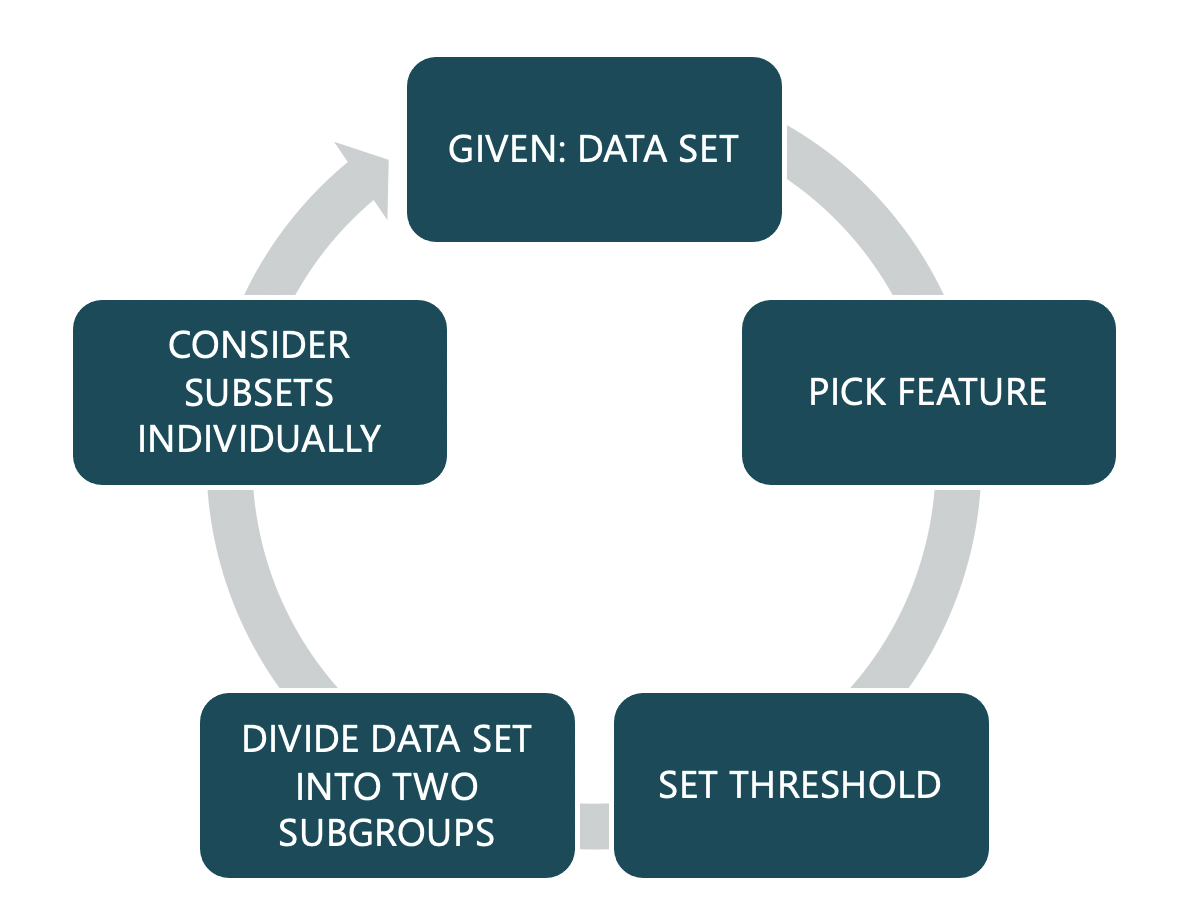
\includegraphics[scale=0.55]{BDT2.png}\label{fig:fig2}
 \caption{The process of buidling a BDT.}
 \end{figure}


 The decision for a specific feature while building a BDT can greatly influence the outcome since the generated subgroups will be completely different. That is why there is a need for a way to assess the most efficient way of splitting the data. For that, the information entropy and information gain are used. The entropy describes the level of information of a variable (\ref{fig:fig3}). The information gain compares two entropies and calculates the difference(\ref{fig:fig4}). The idea is to test every attribute as a possible option for a split node and calculate which attribute would yield the highest gain in information after the split. 

\begin{centering}
   \begin{equation}\label{fig:fig3}
      H(X)= - \sum_{i=1}^{n}P(x_i)\log_2{P(x_i)}
   \end{equation}  
\end{centering}
 
\begin{centering}
   \begin{equation}\label{fig:fig4}
      Information Gain = Entropy(Parent) - Average Entropy(Children)
   \end{equation}  
\end{centering}


 \subsubsection{Example BDT\label{sec:sec2-1-3}}
 Given a table of sample data: \\
 
 
 \begin{table}[]
   \begin{tabular}{|l|l|l|l||l|}
      \hline
      Temperature & Rain & Windy & Humidity & Go outside? \\
    \hline
    \hline
    High & Yes & True & High & No \\
    \hline
    Low& No & False & Low & Yes \\
    \hline
    Low& No & True & Low & No \\
    \hline
    High& No & False &  High& Yes \\
    \hline
    High&  Yes& False & Low & No \\
    \hline
    Low& Yes & True & Low & No \\
    \hline
    High& No &  False&  Low& Yes \\
    \hline
    Low&  Yes& True & High & No \\
    \hline
    Low&  No& True & High &  Yes\\
    \hline
    Low&  No&  False& Low & Yes \\
    \hline
    High&  Yes& True & High &  No\\
    \hline
    High&  Yes&  False& Low & No \\
    Low&  No& True& High & Yes\\
    \hline
    High& Yes & False & High & No\\
    \hline
   \end{tabular}
   \label{fig:fig5}
   \caption{A BDT can be built from a table like such.}
   \end{table}

 
 In order to decide which attribute to pick for the root node the information gain must be calculated for all of them (Temperature, Rain, Windy, and Humidity). For example splitting with Temperature would look like this: \\

 First, we need to calculate the entropy of the complete table. 

\begin{equation}\label{fig:fig8}
   H(X)= - \biggl[\frac{6}{14}\log_2(\frac{6}{14}+\frac{8}{14}\log_2(\frac{8}{14})\biggr]=0,9852
\end{equation}  

 If we were to split at Temperature, the table would be divided into two groups, one with high temperature and one with low temperature. As it has a binary result there is no need to calculate a threshold. Now the entropy for both of these subgroups needs to be calculated individually. The information gain for Temperature is the difference resulting from the complete entropy minus the average entropy of the newly generated subgroups. In this case the information gain is $0.01615$. 

 \begin{equation}\label{fig:fig7}
   \begin{split}
   Temperature=high: H(2,5)= -\biggl[\frac{2}{7}\log_2(\frac{2}{7}+\frac{5}{7}\log_2(\frac{5}{7})\biggr]=0,8631
   \\
   Temperature=low: H(4,3)= -\biggl[\frac{4}{7}\log_2(\frac{4}{7}+\frac{3}{7}\log_2(\frac{3}{7})\biggr]=0,9852
   \\
   Gain: H(2,5)= -\biggl[\frac{7}{14}H(2,5)+\frac{7}{14}H(4,3)\biggr]=0,01615
\end{split}
\end{equation}  

Since the information gain is the value that needs to be maximized the information gain is calculated for the remaining attributes as well. For the root node the attribute is selected that yields the highest information gain. In this case: Rain. 
Having split the data with rain, two subgroups are created (Table 2). One with all Rain values 'Yes' and one with 'No' Rain. Selecting the attribute for the next split node for a subgroup proceeds exactly like with the root node only with a smaller set of data.


\begin{table}[h!]
   \begin{tabular}{|l|l|l|l||l|}
      \hline
      Temperature & Rain & Windy & Humidity & Go outside? \\
    \hline
    \hline
    High & Yes & True & High & No \\
    \hline
    High&  Yes& False & Low & No \\
    \hline
    Low& Yes & True & Low & No \\
    \hline
    Low&  Yes& True & High & No \\
    \hline
    High&  Yes& True & High &  No\\
    \hline
    High&  Yes&  False& Low & No \\
    \hline
    High& Yes & False & High & No\\
    \hline
   \end{tabular}
   \label{fig:fig101}
   \end{table}

   \begin{table}[h]
      \begin{tabular}{|l|l|l|l||l|}
      \hline
         Temperature & Rain & Windy & Humidity & Go outside? \\
       \hline
       \hline
      Low& No & False & Low & Yes \\
      \hline
      Low& No & True & Low & No \\
      \hline
      High& No & False &  High& Yes \\
      \hline
      High& No &  False&  Low& Yes \\
      \hline
      Low&  No& True & High &  Yes\\
      \hline
      Low&  No&  False& Low & Yes \\
      \hline
      Low&  No& True& High & Yes\\
      \hline
      \end{tabular}
      \label{fig:fig102}
      \caption{The two generated subgroups when splitting with Rain at the root node.}
      \end{table}

 The subgroups are recursively divided as long as there are differences in the subgroups decisions. When this is the case leaf nodes are created to label the inserted vector. If all leaf nodes have been created, the final tree is completely trained. In this case the Temperature is not essential for the decision making process.

 
 \begin{figure}[H]
    \centering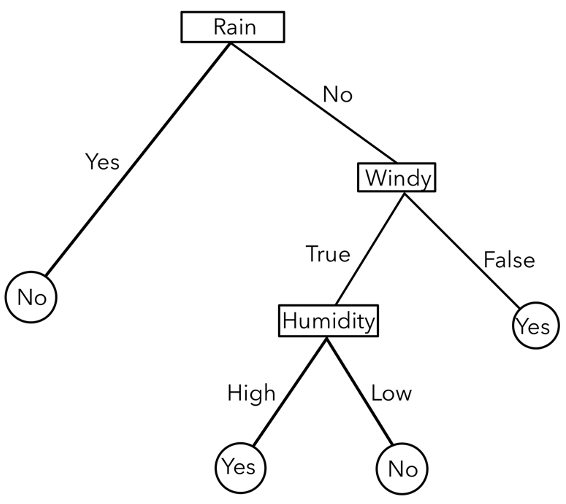
\includegraphics[scale=0.55]{BDT11.png}\label{fig:fig11}
    \caption{The final BDT.} 
 \end{figure}



 \subsubsection{Testing a BDT\label{sec:sec2-1-4}}
 After building a BDT, it has to be ensured that it is working correctly and classifies properly. Therefore not all data is used for building the tree, but a part is saved for testing purposes. Now that the BDT is built, we can pick samples of the test data and insert it into the BDT. As this is a supervised learning method, the result is already known and can thereby be compared with the tree's yielded outcome. If it is correct, the tree is working fine.  

 \subsubsection{Pro and Cons of BDT\label{sec:sec2-1-5}}
 A BDT can be used to classify and label data vectors, which can help many problems. As it is not limited to categorical values for classification but can also work with numerical values, a BDT can also predict future values through regression curves. Furthermore, the technique and structure of a BDT and its decision finding process is intuitive and visualizable. Additionally, the data used only requires little data pre-processing. The problem with BDTs is that small changes in data can heavily affect the outcome of the decision. If the tree internalizes every detail of the training data, it can overfit. That means that the BDT does not reflect the general input data but has adapted to the training data. For instance: If an algorithm was given scans of tumors that are compared to all other existing tumor scans rather dark, then the BDT will set this as the general intensity of a tumor scan. Thereby brighter parts of tumor scans that the BDT has not seen will not be classified as a tumor. In order to face that issue, Random Forests have been introduced. 

 \subsection{Random Forest\label{sec:sec2-2}}
   RDF overcome the obstacle of overfitting through the use of multiple BDTs and randomness. A tested vector is inserted into multiple trees, which all yield a decision for that vector. One way to determine the overall final decision is to decide by a majority vote. An individual tree might be overfit at some points in the forest, however, this does not influence the final decision too much. One way to increase accuracy through multiple trees is called Bagging.

 \subsubsection{Bagging\label{sec:sec2-2-1}}
 While building a random forest, several trees have to be built. When for each tree, only a subset of the training data is being used, it is called Bagging. Thereby randomness is introduced in the procedure and improves the reliability of the decision. Additional to bagging there are similar approaches like randomized node optimization which uses a subset of features instead of a subset of training data.  
 
 \begin{figure}[H]
 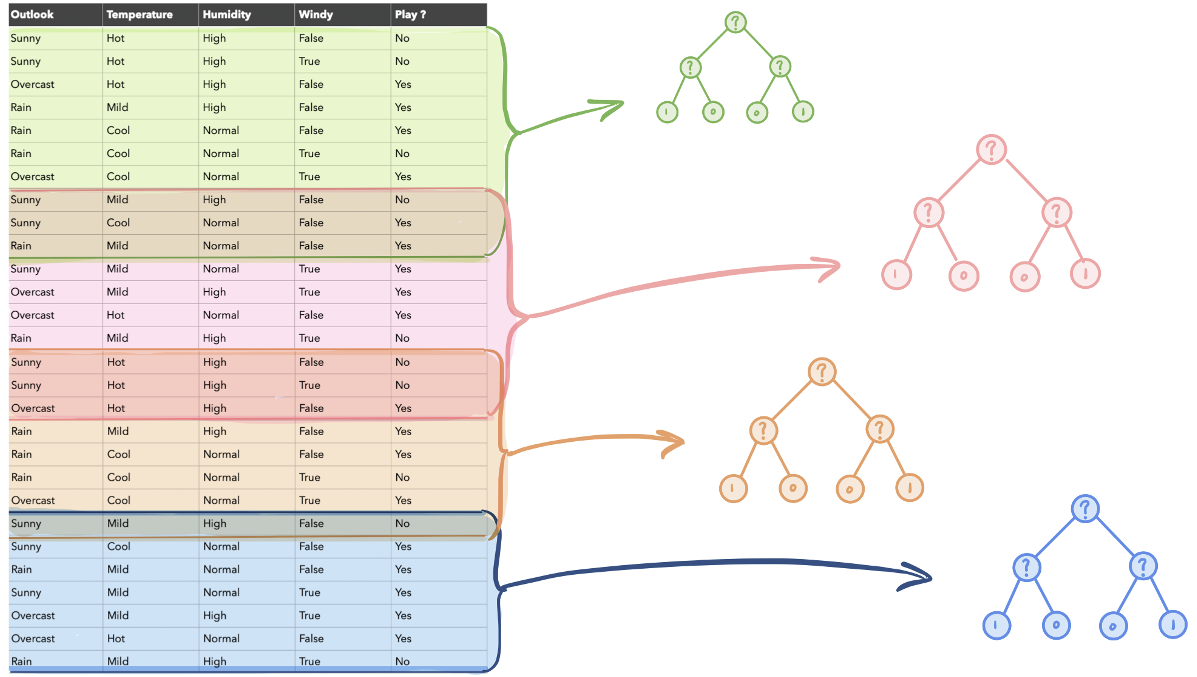
\includegraphics[scale=0.4]{BDT12.png}\label{fig:fig12}
 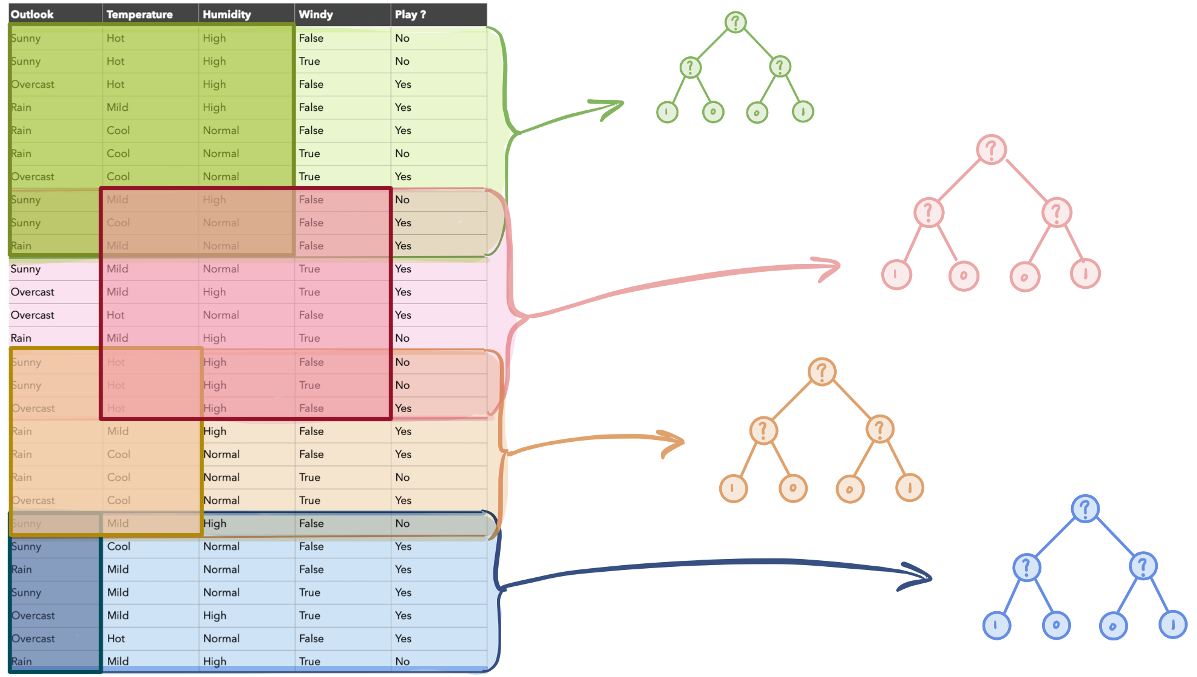
\includegraphics[scale=0.4]{BDT13.png}\label{fig:fig13}
 \caption{Bagging(left): Each tree is trained by individual data set, Bagging +randomized note optimization (right) Each tree is trained by an individual set of data and features.}

 \end{figure}

RDF can be described and influenced by many parameters like the size of the forest meaning the number of trees. Many papers state that the larger a forest gets, the more accurate its decision will be, up to a certain cutoff. Another aspect is the depth of an individual tree so the number of split nodes it contains. Sometimes deep trees can be prone to overfit, which can be faced with using more training data. Also the number of smaples used in training a RDF can be important to consider.


\section{Application\label{sec:sec3}}

 \subsection{Goal of the Paper\label{sec:sec3-1}}
 The paper aims to develop a reliable procedure based on machine learning ensembles to detect tumors on MRI scans in an early stage and segment them. For the execution of the experiment, 12 records from the Multimodal Brain Tumor Segmentation Challenge(BRATS) Data Set were used. Within the 2012 MICCAI conference the BRATS provided manually pro-delinated records next to realistically generated synthetic brain tumor datasets. In this experiment each record belongs to one patient and contains four different MRI scans (T1, T2, T1C, FLAIR), which display the same brain in different ways. Each record consists of approximately 1.5 Mio feature vectors. There is a truth image containing expert annotations for either an active tumor or edema cells for every volume. The algorithm is supposed to separate tumor cells, edema cells, and negative cells.

 \subsection{Data and Pre-Processing\label{sec:sec3-2}}
 In order to address a voxel, a feature vector is generated. This process is visualized in the following graphic.\\
 
 \begin{center} $T[x,y,z] = \biggl[T1[x,y,z], T2[x,y,z], T1C[x,y,z], FLAIR[x,y,z]\biggr]$\end{center}

 \begin{figure}[H]
 \centering 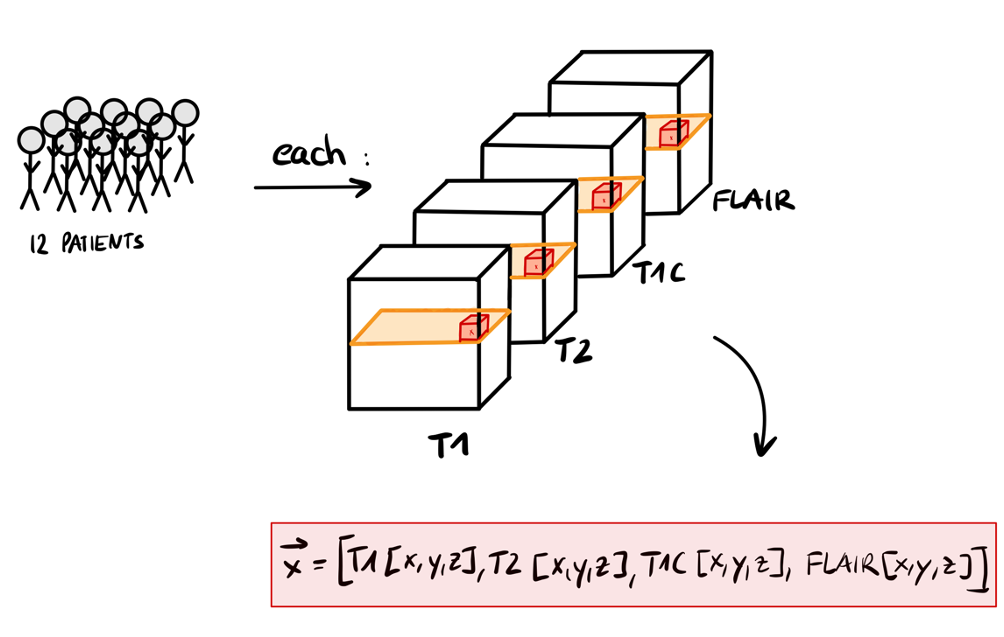
\includegraphics[scale=0.6]{BDT14.png}\label{fig:fig14}
 \caption{The Feature vector is generated to address a specific cell in all four cells.}
 \end{figure}

 Before the data is used in training and testing BDTs and RDFs, it needs to be pre-processed and translated into a shared format the BDT understands. The first step is the histogram normalization. A histogram displays the number of occurences of specific intensity values. In this case, the middle 50$\%$ of the data is supposed to be located between the intensity values of $600$ and $800$. Also, the minimum value of $200$ and the maximum value of $1200$ are set as boundaries. The second step involves the neighborhood of a considered voxel. Since the feature vector does not include any information regarding the voxel's location, two more features have to be computed for each scan. The new feature vector will thereby consist of 12 elements. For the computation of the first added feature, all direct neighbor voxels in a $3 \times 3 \times 3$-sized Cube are considered. The average intensity value of them is the first new feature value of the vector. The second feature is computed based on the average intensity value of the eight closest voxels of that slice and two closest ones from the neighboring slices. 

 \begin{figure}[H]
 \centering 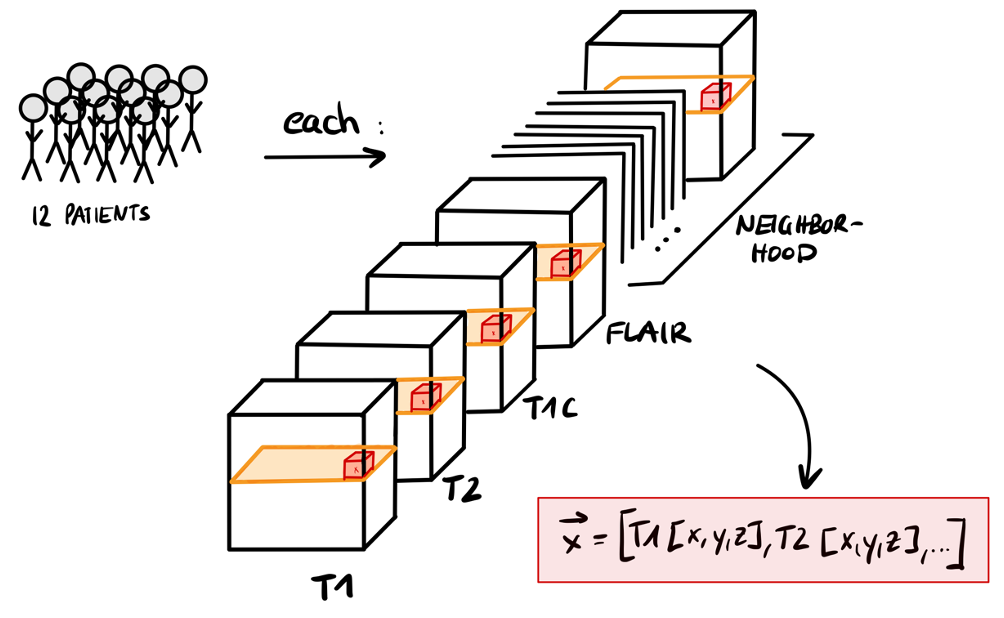
\includegraphics[scale=0.5]{BDT15.png}\label{fig:fig15}
 \caption{The updated Feature vector contains twelve elements.}
 \end{figure}



 The last step of pre-processing excludes the missing voxels from the average calculations for the neighborhood. Null values would distort the result and must thereby be ignored for the average intensity value. 

 \subsection{Training and Testing\label{sec:sec3-3}}
 The data is now ready to be used for training BDTs. Compared to the above mentioned example the attributes are now T1, T2, etc. As 1.5 Mio vectors are too many to use on training, the tree samples have to be selected. In the experiment 300 samples of each label are selected.
 
 \subsection{post-processing\label{sec:sec3-4}}
 Even though the BDT and RDF classify most of the voxels reliably, there are usually some negative cells labeled as tumor or edema due to the great variety of normal tissues they can belong to. In order to correct falsely labeled positives for each tumor and edema voxel, a 250-voxel neighborhood is defined. The number of voxels which are labeled the same is then compared with a pre-defined threshold, which value is debatable. If the voxel intensity in question is less than the average intensities, it is relabeled into a negative voxel; it remains the same if it is higher.

\section{Experiments and Results\label{sec:sec4}}

 In the paper different experiments were conducted. The tool used to compare their accuracy is called Dice Score which mapes the accuracy on a scale from zero to one where one means very accurate. 
 The first achievement of this paper's experiment is that the size of a sample used for training a BDT influences the accuracy of the decision. In Figure 7 the increase of the Dice Score is shown per rising number of test cases. That shows that increasing the number of samples up to a certain point between 1000 and 5000, leads to a rise in accuray.
 
 \begin{figure}[H]
 \centering 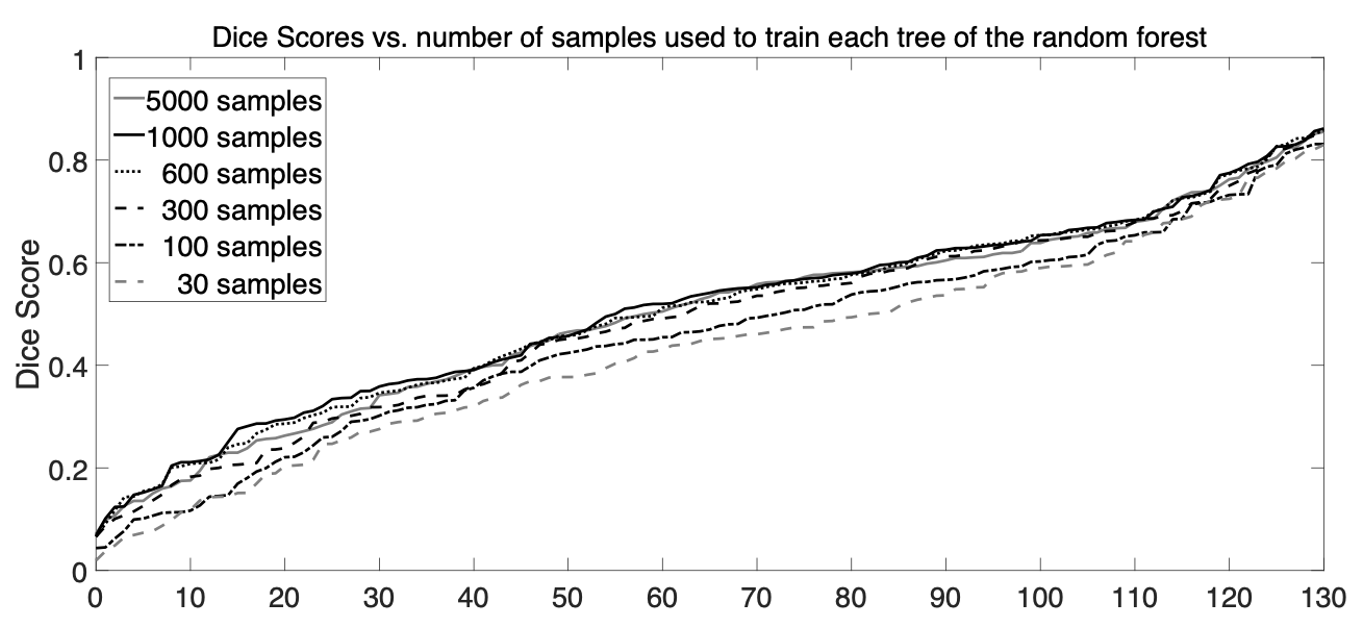
\includegraphics[scale=0.5]{BDT16.png}\label{fig:test}
 \caption{The sample size can influence the Dice Score}
 \end{figure} 

 The second result shows the dice scores when training a RDF with volume $a$ and testing with volume $b$ and another training with volume $b$ and testing with $a$. The table does not shown symmetry regarding training and testing with volumes. It should be emphasized that the right site draws a higher overall score. 

 \begin{figure}[H]
 \centering 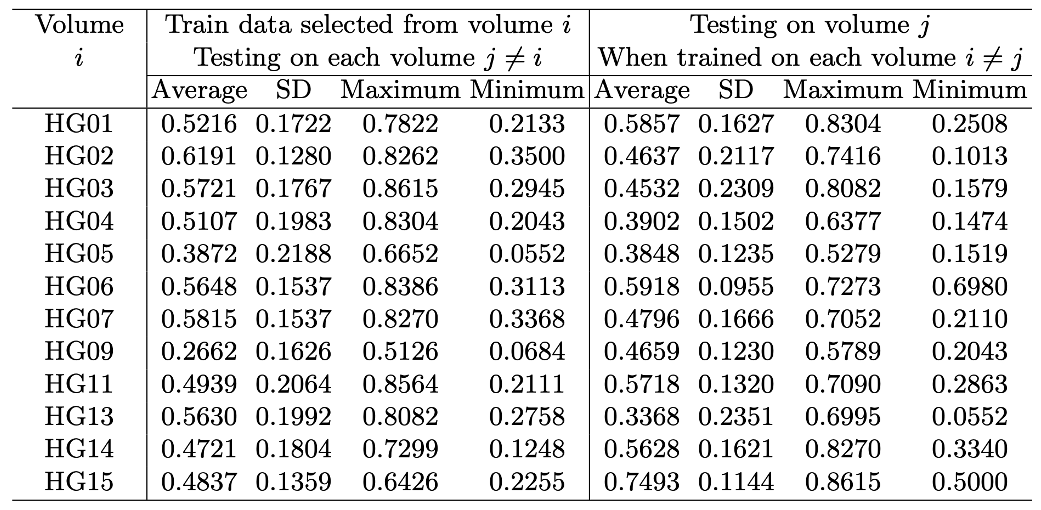
\includegraphics[scale=0.7]{BDT17.png}\label{fig:fig17}
 \caption{Training and testing is not symmetric}
 \end{figure} 

 The following charts concern the effect of post-processing. Looking at the blue diagrams, it becomes clear that Post-Processing can be highly beneficial for increasing the Dice Score. In the lower graphs, the Dice Score is drawn depending on how the threshold for the 250-voxel neighborhood. A threshold around 200 yields the most promising results. 


 In Figure 9 two MRI scans are shown, one without Post-processing (left) and one with Post-Processing (right). What stands out is that Post-Processing finds non-affected cells in between tumor cells that would have been labeled positive. That gives a more detailed and concise scan, which can facilitate and enhance the tumor's treatment. 

 \begin{figure}[H]
 \centering 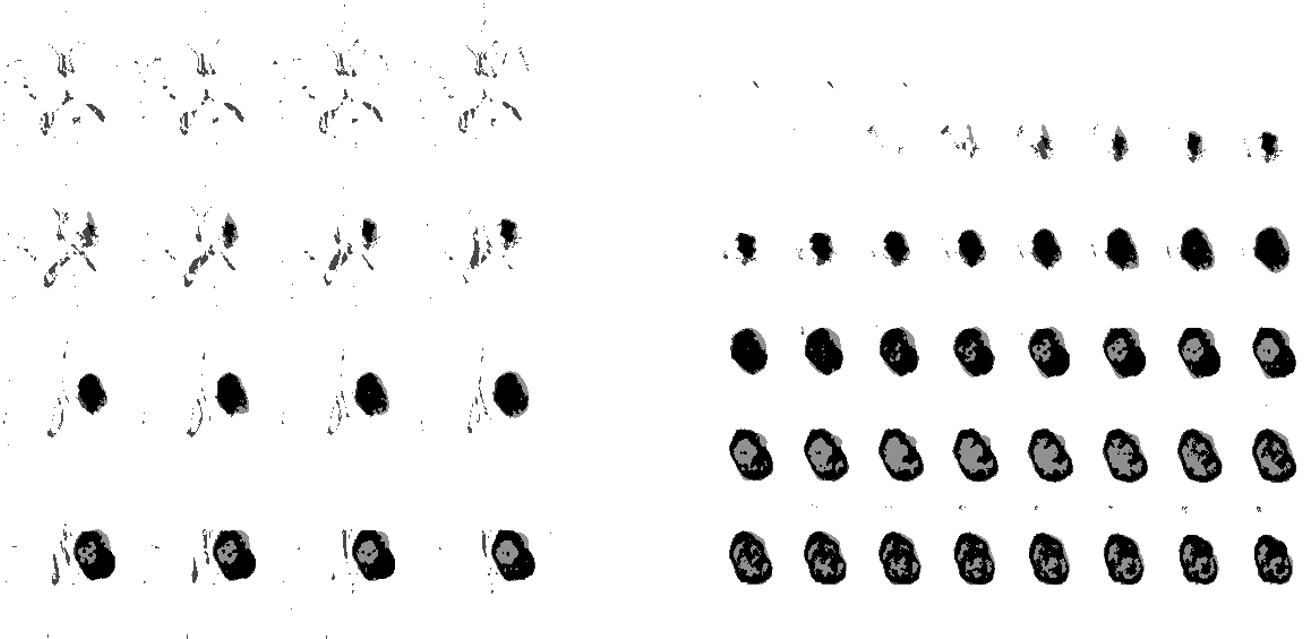
\includegraphics[scale=0.5]{BDT19.png}\label{fig:fig19}
 \caption{MRI scan without Post-Processing (left), MRI scan with Post-Processing (right). Black areas show true positives and gray areas false positives.}
 \end{figure} 

\section{Conclusion\label{sec:sec5}}

  In conclusion, the automatic detection and segmentation of brain tumors using the RDF approach yields acceptable results and can well be envisioned in future clinical applications. However the RDF must be applied under the right conditions like the right number of volumes used to train and test it. Also other parameters like the size of samples can affect the accuracy of the Forests decision deeply. The future development and application will probably consist of multiple clusters of trees, each trained with individually dedicated volumes. Methods like bagging or random node optimization must be chosen carefully befor emplyoing a BDT. This papers experiment showed that it will be possible to apply Random Forests in the future detection of tumors. 


\section{References\label{sec.sec5}}


%--------------------------------------------------
% Example of a table
%--------------------------------------------------


\begin{table}[H]
 \footnotesize
% \caption{\label{tab:table1} Topics of the presentations \textbf{two years ago}.}
 \vspace{1ex}
 \centering 
 \begin{tabular}{p{2.5cm}p{8.7cm}p{2.8cm}}
 \toprule
 \textbf{Author} & \textbf{Literature} & \textbf{Release} \\
 \midrule
 Zoltán Kapás & Automatic Detection and Segmentation of Brain Tumor Using Random Forest Approach & 2016 \\
 Ralf Moeller & Vorlesung Einführung in Web und Data Science & 2018 \\
 A. Criminisi & Decision Forests for Classification, Regression, Density, Esimation, Manifold, Learning and Semi-Supervised Learning & 2011 \\
 Kahild Usman & Brain tumor classification from multi-modality MRI using wavelets and machine learning & 2017 \\
 Bjoern Menze&Multimodal Brain Tumor Segmentation Challenge&2012\\
 D. Zikic&Context-sensitive Classification Forests for Segmentation of Brain Tumor Tissues&2012\\
 S.Bauer&Segmentation of Brain Tumor Images Based on Integrated Hierarchical Classification and Regularization&2012\\
 T.Riklin Raviv&Multi-modal Brain Tumor Segmentation via Latent Atlases&2012


 %\bottomrule
 \end{tabular}
 \vspace{2ex}
\end{table}


%==================================================
%\newpage
%\bibliographystyle{plain}
%\bibliographystyle{elsarticle-harv}
%\footnotesize\bibliography{bib}


\end{document}

